% !TEX root = knottedMain.tex
\documentclass[varwidth=\maxdimen]{standalone}

\usepackage{mathtools,amssymb,mathrsfs,dutchcal,upgreek,faktor,accents,etoolbox,multicol}
\usepackage[dvipsnames]{xcolor}
\definecolor{mygreen}{RGB}{	8,156,79 }
\usepackage{tikz,tikz-cd}
\usetikzlibrary{patterns,knots,arrows.meta,decorations.markings}
\tikzset{>={Straight Barb[scale=0.85]}}
\tikzcdset{
  cells={font=\everymath\expandafter{\the\everymath\displaystyle}},
  arrow style=tikz,
  diagrams={>={Straight Barb[scale=0.85]}},
  every label/.append style = {font = \small}
}


\begin{document}
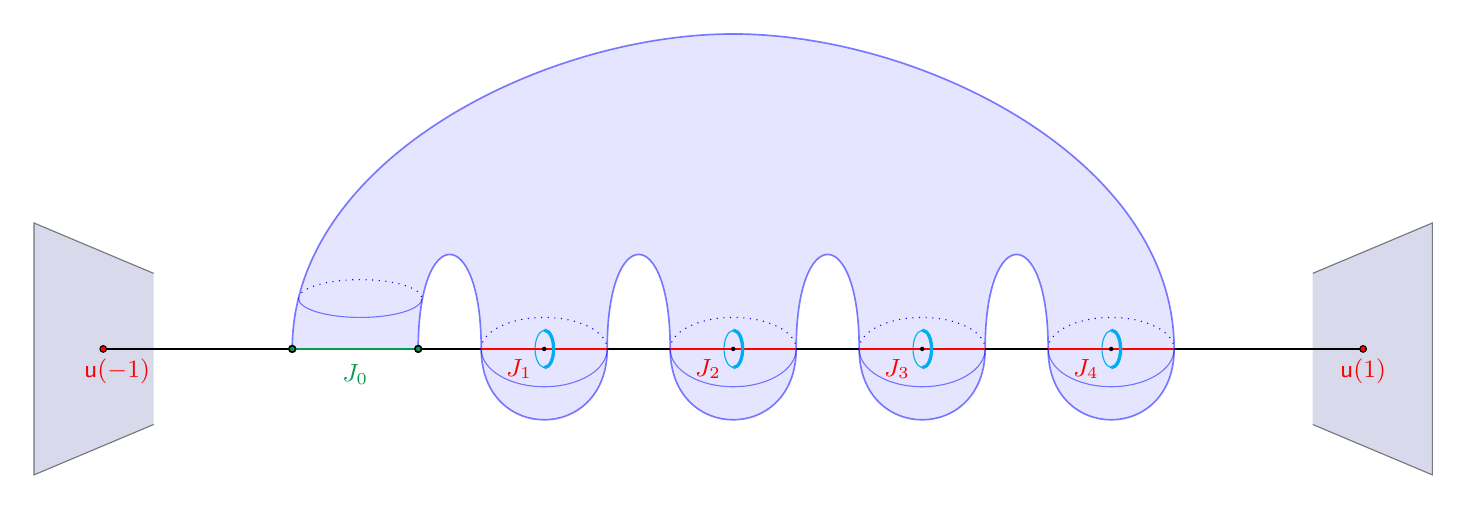
\begin{tikzpicture}[scale=0.8]
    \clip (-2.2,-2.1) rectangle (20.2,5.1);
    % boundary of M
    \fill[blue!50!black,opacity=0.15,draw=black,draw opacity=0.5]
        (18.2,-1.2) -- (20.1,-2) -- (20.1,2) --  (18.2,1.2) ;
    \fill[blue!50!black,opacity=0.15,draw=black,draw opacity=0.5]
        (-.2,1.2) -- (-2.1,2) -- (-2.1,-2) -- (-.2,-1.2) ;
    \draw[semithick]
        (-1,0) -- (19,0) ;

    \fill[color=blue!20!,opacity=0.5,draw=blue,semithick]
        (2,0) to[out=90,in=180,distance=3cm] 
        (9,5) to[out=0,in=90,distance=3cm] 
        (16,0)  to[out=-90,in=-90,distance=1.5cm]
        (14,0)  to[out=90,in=90,distance=2cm]
        (13,0) to[out=-90,in=-90,distance=1.5cm]
        (11,0)  to[out=90,in=90,distance=2cm]
        (10,0) to[out=-90,in=-90,distance=1.5cm]
        (8,0)  to[out=90,in=90,distance=2cm]
        (7,0) to[out=-90,in=-90,distance=1.5cm]
        (5,0)  to[out=90,in=90,distance=2cm]
        (4,0) --
        (2,0);
    % spheres
    \foreach \y/\i/\j in {6/0,9/1,12/2,15/3}{
        \draw[blue,opacity=0.5] (\y-1,0) arc (180:360:1cm and 0.6cm);
        \draw[blue,dotted] (\y-1,0) arc (180:0:1cm and 0.5cm);
        % \shade[ball color=blue!20!,opacity=0.3] (\y,0) circle (1cm);
        % \draw[blue,semithick] (\y,0) circle (1cm);
        % \draw (\y,-1) node[below=2pt]{$\mathbb{S}_{\i}$};
        }
     % vertical arcs
    \foreach \x in {6,9,12,15}{
        \draw[cyan,thin]
            (\x,0.3) to[out=-165,in=165, distance=0.2cm] (\x,-0.3);
    }
        
    \draw[blue,opacity=0.5] (2.1,0.8) arc (180:360:0.98cm and 0.3cm);
    \draw[blue,dotted] (2.1,0.8) arc (180:0:0.98cm and 0.3cm);
    
    \draw[mygreen, thick]
            (2,0) -- (4,0) %node[fill=mygreen!30,draw, pos=0.5]{}
            (3, 0) node[below=2pt]{\small$J_0$};
    \fill[mygreen,draw=black,semithick] 
        (2,0) circle (1.5pt) (4,0) circle (1.5pt);


    \fill[red,draw=black]
        (-1,0) circle (1.5pt) (-0.78,0) node[below]{\small$\mathsf{u}({-}1)$}
        (19,0) circle (1.5pt) node[below]{\small$\mathsf{u}(1)$};
    \draw[semithick,red]
        (5,0)--(7,0) node[pos=0.3,below]{\small$J_1$}
        (8,0)--(10,0) node[pos=0.3,below]{\small$J_2$}
        (11,0)--(13,0) node[pos=0.3,below]{\small$J_3$}
        (14,0)--(16,0) node[pos=0.3,below]{\small$J_4$};

             % vertical arcs
    \foreach \x in {6,9,12,15}{
        \draw[cyan,very thick]
            (\x,0.3) to[out=-5,in=5, distance=0.2cm] (\x,-0.3);
        \fill (\x,0) circle (1pt) %node[below]{\small$u_{\i}$}
        ;
    }
\end{tikzpicture}

\end{document}